\documentclass[12pt,a4paper]{article}

\usepackage{mathpazo}

\usepackage[utf8x]{inputenc}
\usepackage{bm}
\usepackage{tikz}
%\usepackage{tkz-euclide}
\usetikzlibrary{positioning,through,calc,intersections,arrows.meta}
\usetikzlibrary{external}
\tikzexternalize[prefix=tikz/]
\tikzset{>=stealth} % Use stealth arrows
%\usetkzobj{all}

\textwidth=155mm
\textheight=235mm
\topmargin=0pt
\headheight=0pt
\oddsidemargin=5mm
\headsep=0pt
\parindent=0pt
\renewcommand{\baselinestretch}{1.1}
\setlength{\parskip}{0.3\baselineskip plus 1pt minus 1pt}

\begin{document}
\thispagestyle{empty}

\begin{center}

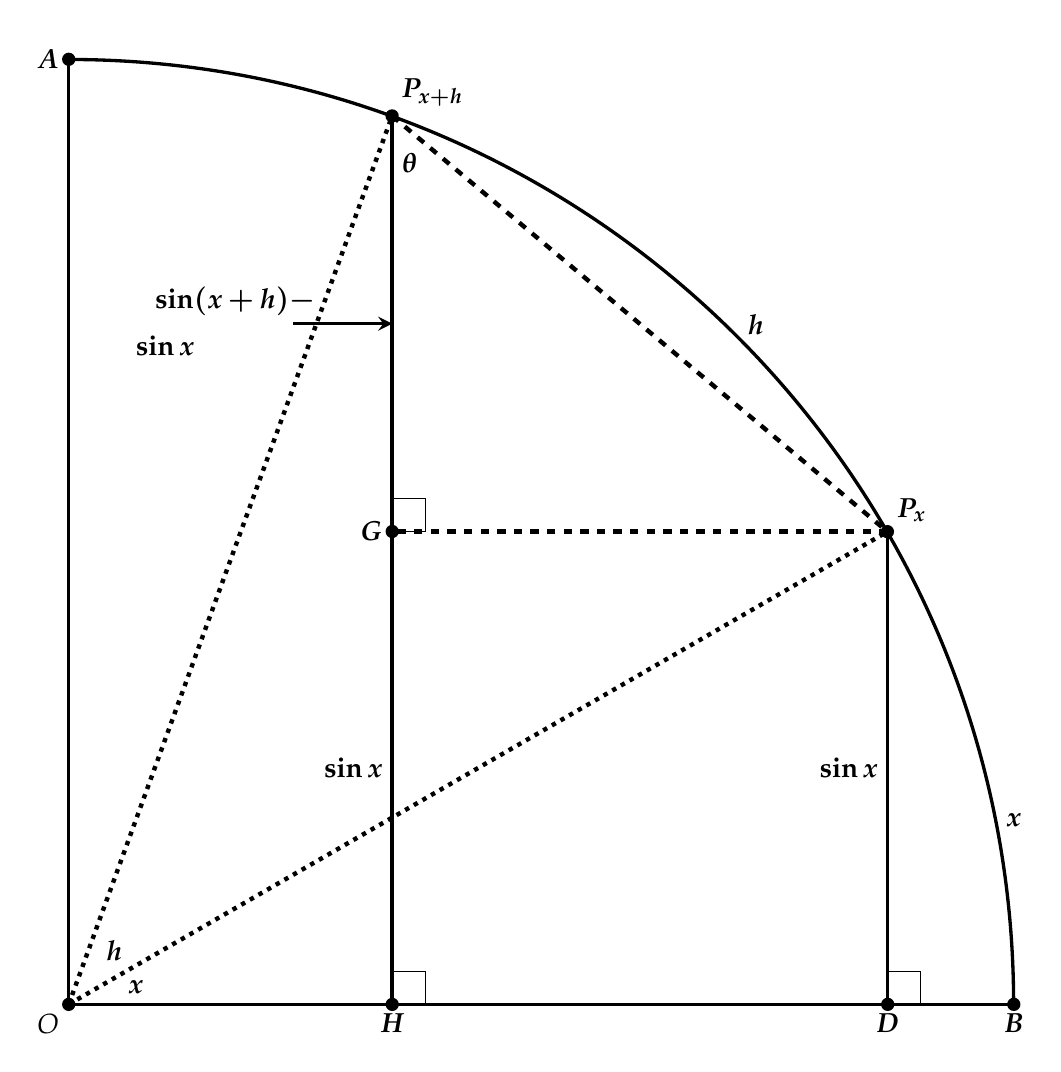
\begin{tikzpicture}[scale=1.2]
\coordinate (O) at (0,0);
\coordinate (A) at (0,10);
\coordinate (B) at (10,0);
\fill (O) circle (2pt) node[below left] {$O$} node[right,xshift=18pt,yshift=6pt] {$\bm{x}$} node[above right,xshift=10pt,yshift=12pt] {$\bm{h}$};
\fill (A) circle (2pt) node[left] {$\bm{A}$};
\fill (B) circle (2pt) node[below] {$\bm{B}$};

\draw[very thick,name path=axes] (B) -- (O) -- (A);
\draw[very thick,name path=arc] (10,0) arc[start angle=0, end angle=90, radius=10] node[very near start,right] {$\bm{x}$} node[midway,right,yshift=4pt] {$\bm{h}$};

\path[name path=px] (O) -- (30:11);
\path [name intersections={of=arc and px,by={Px}}];
\fill (Px) circle (2pt) node[above right] {$\bm{P_x}$};

\draw[very thick,name path=pxd] (Px) |- (O);
\path [name intersections={of=pxd and axes,by={D}}];
\fill (D) circle (2pt) node[below] {$\bm{D}$};

\path[name path=pxh] (O) -- (70:11);
\path [name intersections={of=arc and pxh,by={Pxh}}];
\fill (Pxh) circle (2pt) node[above right] {$\bm{P_{x+h}}$} node[below right,yshift=-10pt] {$\bm{\theta}$};

\draw[very thick,name path=pxh] (Pxh) |- (O);
\path [name intersections={of=pxh and axes,by={H}}];
\fill (H) circle (2pt) node[below] {$\bm{H}$};

\draw[ultra thick,dashed,name path=pxpxh] (Px) -| (Pxh);
\path [name intersections={of=pxh and pxpxh,by={G}}];
\fill (G) circle (2pt) node[left] {$\bm{G}$};

\draw (D) rectangle +(10pt,10pt);
\draw (G) rectangle +(10pt,10pt);
\draw (H) rectangle +(10pt,10pt);

\draw[ultra thick,dotted] (O) -- (Pxh);
\draw[ultra thick,dotted] (O) -- (Px);
\draw[ultra thick,dashed] (Pxh) -- (Px);

\path (D) -- node[left] {$\bm{\sin x}$} (Px);
\path (H) -- node[left] {$\bm{\sin x}$} (G);
%\path (G) -- node[left] {$\bm{\sin(x+h)\!-\!\sin x}$} (Pxh);
\path (G) -- node[xshift=-24pt,yshift=+8pt,left] {$\bm{\sin(x+h)-}$} (Pxh);
\path (G) -- node[xshift=-68pt,yshift=-8pt,left] {$\bm{\sin x}$} (Pxh);
\draw[<-,very thick] ($(G)!.5!(Pxh)$) -- +(-30pt,0);
\end{tikzpicture}

\end{center}

\end{document}

In the following diagram, $x$ is the length of an arc of the unit circle from $B$ on the $x$-axis to point $P_x$ (and it is also the measure in radians of the angle that the arc subtends). Similarly, $h$ is the length of an arc somewhat farther along the arc from $P_x$ to $P_{x+h}$. $P_xD$ and $P_{x+h}H$ are perpendicular to the $x$-axis and $P_xG$ is perpendicular to $P_{x+h}H$. We are interested in the angle $\theta$.

\begin{center}

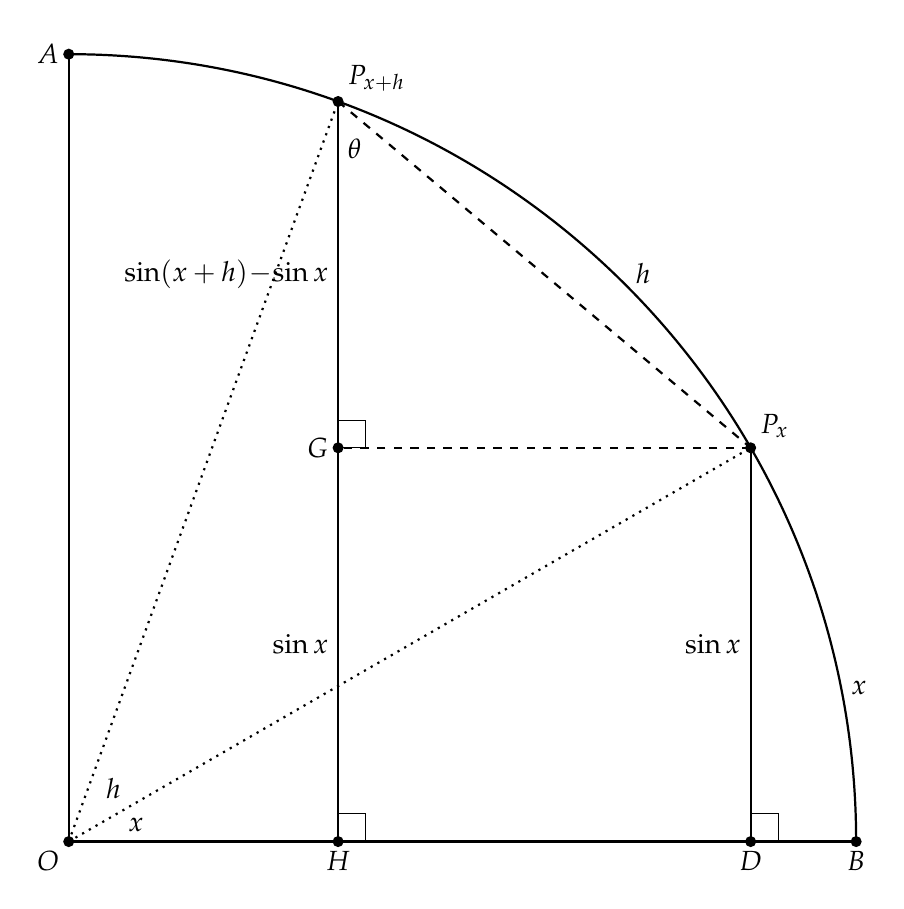
\begin{tikzpicture}
\coordinate (O) at (0,0);
\coordinate (A) at (0,10);
\coordinate (B) at (10,0);
\fill (O) circle (2pt) node[below left] {$O$} node[right,xshift=18pt,yshift=6pt] {$x$} node[above right,xshift=10pt,yshift=12pt] {$h$};
\fill (A) circle (2pt) node[left] {$A$};
\fill (B) circle (2pt) node[below] {$B$};

\draw[thick,name path=axes] (B) -- (O) -- (A);
\draw[thick,name path=arc] (10,0) arc[start angle=0, end angle=90, radius=10] node[very near start,right] {$x$} node[midway,right,yshift=4pt] {$h$};

\path[name path=px] (O) -- (30:11);
\path [name intersections={of=arc and px,by={Px}}];
\fill (Px) circle (2pt) node[above right] {$P_x$};

\draw[thick,name path=pxd] (Px) |- (O);
\path [name intersections={of=pxd and axes,by={D}}];
\fill (D) circle (2pt) node[below] {$D$};

\path[name path=pxh] (O) -- (70:11);
\path [name intersections={of=arc and pxh,by={Pxh}}];
\fill (Pxh) circle (2pt) node[above right] {$P_{x+h}$} node[below right,yshift=-10pt] {$\theta$};

\draw[thick,name path=pxh] (Pxh) |- (O);
\path [name intersections={of=pxh and axes,by={H}}];
\fill (H) circle (2pt) node[below] {$H$};

\draw[thick,dashed,name path=pxpxh] (Px) -| (Pxh);
\path [name intersections={of=pxh and pxpxh,by={G}}];
\fill (G) circle (2pt) node[left] {$G$};

\draw (D) rectangle +(10pt,10pt);
\draw (G) rectangle +(10pt,10pt);
\draw (H) rectangle +(10pt,10pt);

\draw[thick,dotted] (O) -- (Pxh);
\draw[thick,dotted] (O) -- (Px);
\draw[thick,dashed] (Pxh) -- (Px);

\path (D) -- node[left] {$\sin x$} (Px);
\path (H) -- node[left] {$\sin x$} (G);
\path (G) -- node[left] {$\sin(x+h)\!-\!\sin x$} (Pxh);
\end{tikzpicture}

\end{center}

$\theta$ is the difference between two angles:
\[
\theta=\angle GP_{x+h}P_x= \angle OP_{x+h}P_x - \angle OP_{x+h}H\,.
\]
Since all radii are equal, $\triangle OP_{x+h}P_x$ is isoceles, and since the sum of the angles of a triangle is $\pi$ we have:
\[
\angle OP_{x+h}P_x=\frac{1}{2}(\pi - h)\,.
\]
From the sum of the angles in the right triangle $\triangle OP_{x+h}H$ we have:
\[
\angle OP_{x+h}H = \left(\pi-\frac{\pi}{2}-(x+h)\right) = \left(\frac{\pi}{2}-(x+h)\right)\,.
\]
Therefore:
\[
\theta = \frac{1}{2}(\pi - h) - \left(\frac{\pi}{2}-(x+h)\right) = x+\frac{h}{2}\,.
\]
From the definition of the trigonometric function cosine in the triangle $P_xGP_{x+h}$:
\[
\cos \theta = \frac{\sin(x+h)\!-\!\sin x}{P_{x+h}P_x}\approx \frac{\sin(x+h)\!-\!\sin x}{h}\,,
\]
taking the length of the arc $h$ as an approximation of the chord $P_xP_{x+h}$. The approximation improves are $h$ becomes smaller, so:
\[
\sin' x = \lim_{h\rightarrow 0} \frac{\sin(x+h)\!-\!\sin x}{h} =  \lim_{h\rightarrow 0}\cos \theta = \lim_{h\rightarrow 0} \cos \left(x+\frac{h}{2}\right) = \cos x\,.
\]
\end{document}
